%% LaTeX Beamer presentation template (requires beamer package)
%% see http://bitbucket.org/rivanvx/beamer/wiki/Home
%% idea contributed by H. Turgut Uyar
%% template based on a template by Till Tantau
%% this template is still evolving - it might differ in future releases!

%% Template edited by Panagiotis Adamopoulos {padamopo}@stern.nyu.edu

\documentclass[aspectratio=169]{beamer}
 
\mode<presentation>
{
\usetheme{NYU}

\setbeamercovered{transparent}
}

\usepackage[english]{babel}
\usepackage[latin1]{inputenc}
\usepackage[scaled=.90]{helvet}
\usepackage{courier}
\usepackage[T1]{fontenc}
\usepackage{comment}
%usepackage{appendixnumberbeamer}
\usepackage{amsmath}
\usepackage{bm}
\usepackage{pgfpages}
\usepackage{pgfplots}
\pgfplotsset{compat=1.18}
\usepackage[breakable, skins]{tcolorbox}
\usepackage{booktabs}
\usepackage{listings}
\definecolor{lstbg}{rgb}{0.97,0.97,0.97}
\definecolor{lstkw}{rgb}{0.13,0.29,0.53}
\definecolor{lststr}{rgb}{0.16,0.40,0.16}
\definecolor{lstcom}{rgb}{0.55,0.55,0.55}
\lstdefinestyle{pystyle}{
	language=Python,
	basicstyle=\ttfamily\fontsize{5}{5.7}\selectfont,
	backgroundcolor=\color{lstbg},
	keywordstyle=\color{lstkw}\bfseries,
	stringstyle=\color{lststr},
	commentstyle=\color{lstcom}\itshape,
	showstringspaces=false,
	breaklines=true,
	breakatwhitespace=false,
	columns=flexible,
	keepspaces=true,
	frame=single,
	framesep=2pt,
	xleftmargin=4pt,
	xrightmargin=2pt,
	aboveskip=2pt,
	belowskip=2pt,
}
\lstset{style=pystyle}

% Roadmap boxes for Part (a) sidebar
\newcommand{\rmboxon}[2]{%
	\begin{tcolorbox}[enhanced, rounded corners,
		colback=#1!22, colframe=#1!65!black,
		boxrule=0.8pt,
		width=\linewidth, boxsep=1pt,
		left=5pt, right=5pt, top=2pt, bottom=2pt,
		before skip=2pt, after skip=2pt,
	]
	\scriptsize\textbf{#2}
	\end{tcolorbox}%
}
\newcommand{\rmboxoff}[1]{%
	\begin{tcolorbox}[enhanced, rounded corners,
		colback=gray!6, colframe=gray!35,
		boxrule=0.5pt,
		width=\linewidth, boxsep=1pt,
		left=5pt, right=5pt, top=2pt, bottom=2pt,
		before skip=2pt, after skip=2pt,
	]
	\scriptsize\textcolor{gray!55!black}{#1}
	\end{tcolorbox}%
}
% citations
\usepackage{natbib}
\bibpunct{(}{)}{;}{a}{,}{,}
\def\citeapos#1{\citeauthor{#1}'s (\citeyear{#1})}
\renewcommand{\bibsection}{\subsubsection*{\bibname } }

\input{latex-math/basic-math.tex}
\input{latex-math/basic-ml.tex}
\input{latex-math/ml-infotheory.tex}

\newcommand{\kld}[1]{D_{KL}\left(#1\right)}
\newcommand{\Ef}{\mathbb{E}_f}
\newcommand{\Varf}{\mathrm{Var}_f}

\title[]{\textbf{Supervised Learning: Exercise of \\ Information Theory Part 1}}

%\subtitle{}

% - Use the \inst{?} command only if the authors have different
%   affiliation.
%\author{F.~Author\inst{1} \and S.~Another\inst{2}}
\author{Yawei Li} 

% - Use the \inst command only if there are several affiliations.
% - Keep it simple, no one is interested in your street address.
\institute[LMU]
{
\\
  \texttt{yawei.li@stat.uni-muenchen.de}
}

\date{May 21, 2026}


% This is only inserted into the PDF information catalog. Can be left
% out.
\subject{Subject}



% If you have a file called "university-logo-filename.xxx", where xxx
% is a graphic format that can be processed by latex or pdflatex,
% resp., then you can add a logo as follows:

% \pgfdeclareimage[height=0.5cm]{university-logo}{university-logo-filename}
% \logo{\pgfuseimage{university-logo}}



% Delete this, if you do not want the table of contents to pop up at
% the beginning of each subsection:
%\AtBeginSubsection[]
%{
%\begin{frame}<beamer>
%\frametitle{Outline}
%\tableofcontents[currentsection,currentsubsection]
%\end{frame}
%}

% If you wish to uncover everything in a step-wise fashion, uncomment
% the following command:

%\beamerdefaultoverlayspecification{<+->}

\begin{document}



\begin{frame}[noframenumbering, plain]
\titlepage

\end{frame}


\begin{frame}{Exercise 1: Kullback-Leibler Divergence}
	\small
	\begin{columns}[T]
	\begin{column}{0.52\textwidth}
		(a) Approximate the binomial $\mathrm{Bin}(n, p)$ with a Gaussian $\mathcal{N}(\mu, \sigma^2)$. To find a suitable fit, investigate the Kullback-Leibler divergence (KLD) in terms of $\thetav = (\mu, \sigma^2)^T$.
		\vspace{4pt}
		\begin{enumerate}
			\setlength\itemsep{4pt}
			\item Write down the KLD for the given setup.
			\item Derive the gradients w.r.t. $\thetav$.
			\item Is there an analytic solution for the optimal parameter setting? If yes, derive the corresponding solution. If no, give a short reasoning.
			\item Independent of the previous exercise, state a numerical procedure to minimize the KLD.
		\end{enumerate}
	\end{column}
	\begin{column}{0.48\textwidth}
		\centering
		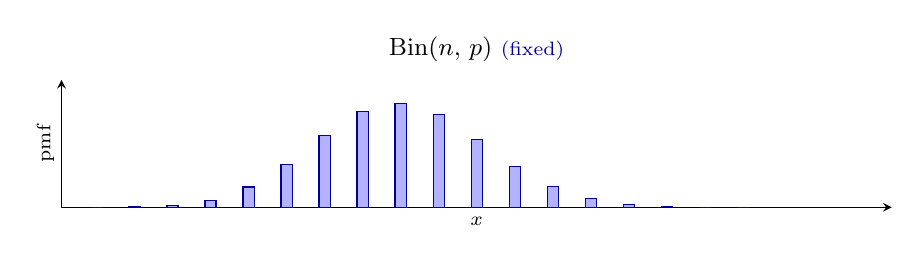
\begin{tikzpicture}
		\begin{axis}[
			width=\linewidth, height=3.2cm,
			title={$\mathrm{Bin}(n,\,p)$ \textcolor{blue!60!black}{\scriptsize (fixed)}},
			title style={font=\small, yshift=-3pt},
			xlabel={$x$}, ylabel={pmf},
			xlabel style={font=\scriptsize, yshift=2pt},
			ylabel style={font=\scriptsize, yshift=-3pt},
			xtick=\empty, ytick=\empty,
			axis lines=left,
			xmin=-0.5, xmax=20.5,
			ymin=0, ymax=0.22,
			enlarge x limits=0.02,
		]
			\addplot[ybar, bar width=4pt, fill=blue!30, draw=blue!60!black]
				coordinates {
					(0, 0.0000366) (1, 0.000487) (2, 0.003087)
					(3, 0.012350) (4, 0.034991) (5, 0.074635)
					(6, 0.124392) (7, 0.165856) (8, 0.179765)
					(9, 0.159791) (10, 0.117142) (11, 0.070995)
					(12, 0.035497) (13, 0.014563) (14, 0.004854)
					(15, 0.001294) (16, 0.000269) (17, 0.0000424)
				};
		\end{axis}
		\end{tikzpicture}

		\vspace{4pt}

		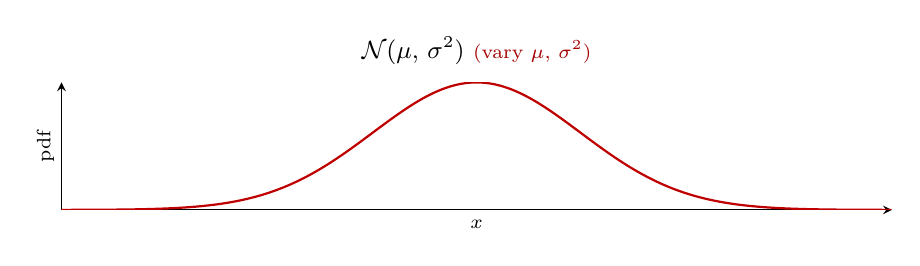
\begin{tikzpicture}
		\begin{axis}[
			width=\linewidth, height=3.2cm,
			title={$\mathcal{N}(\mu,\,\sigma^2)$ \textcolor{red!65!black}{\scriptsize (vary $\mu,\,\sigma^2$)}},
			title style={font=\small, yshift=-3pt},
			xlabel={$x$}, ylabel={pdf},
			xlabel style={font=\scriptsize, yshift=2pt},
			ylabel style={font=\scriptsize, yshift=-3pt},
			xtick=\empty, ytick=\empty,
			axis lines=left,
			ymin=0,
		]
			\addplot[red!75!black, thick, smooth, samples=120, domain=-4:4]
				{1/sqrt(2*pi) * exp(-x^2/2)};
		\end{axis}
		\end{tikzpicture}

		\vspace{4pt}
		{\scriptsize Fix $\mathrm{Bin}(n, p)$; tune $\mu, \sigma^2$ of $\mathcal{N}$ to fit it.}
	\end{column}
	\end{columns}
\end{frame}

\begin{frame}{Solution to Question (a.1)}
	\begin{columns}[T]
	\begin{column}{0.74\textwidth}
		\footnotesize
		Question: Write down the KLD for the given setup.
		\begin{itemize}
			\setlength\itemsep{2pt}
			\item Let $f$ be pmf of $\mathrm{Bin}(n, p)$; we have $\Ef[X] = np$ and $\Varf[X] = np(1 - p)$.
			\item<2-> Let $q$ be the density of $\mathcal{N}(\mu, \sigma^2)$.
		\end{itemize}
		\only<3->{
			The KL divergence between $f$ and $q$ is
			\begin{align*}
				\kld{f \ || \ q}
				&= \Ef \left[ \log \frac{f(X)}{q(X; \thetav)} \right] \\
				&= \underbrace{\Ef \left[ \log f(X) \right]}_{c_1} - \Ef [\log q(X|\thetav)] \\
				&= c_1 - \Ef \left[ \log \left( \frac{1}{\sqrt{2 \pi \sigma^2}} \exp \left( - \frac{1}{2\sigma^2} (X - \mu)^2 \right) \right) \right] \\
				&= c_1 - \Ef \left[ - \underbrace{\tfrac{1}{2} \log(2\pi)}_{c_2} - \tfrac{1}{2} \log (\sigma^2) - \tfrac{1}{2\sigma^2} (X - \mu)^2 \right]
			\end{align*}
		}
	\end{column}
	\begin{column}{0.26\textwidth}
		\vspace{2pt}
		{\scriptsize\textbf{Part (a) roadmap}}
		\rmboxon{blue}{1.\ Write the KLD between binomial $f$ and Gaussian $q$}
		\rmboxoff{2.\ Compute gradients of the KLD w.r.t.\ $\thetav$}
		\rmboxoff{3.\ Find critical points and check the Hessian}
		\vspace{8pt}
		\rmboxoff{4.\ State a numerical procedure to minimize the KLD}
	\end{column}
	\end{columns}
\end{frame}


\begin{frame}{Solution to Question (a.1): Continued}
	\begin{columns}[T]
	\begin{column}{0.74\textwidth}
		\footnotesize
		\begin{align*}
			\kld{f \ || \ q} &= \underbrace{c_1 + c_2}_{c_3}  + \tfrac{1}{2}\log(\sigma^2) + \tfrac{1}{2\sigma^2} \Ef[(X - \mu)^2] \\
			&= c_3 + \log(\sigma) + \tfrac{1}{2\sigma^2} \left( \underbrace{\Ef[X^2]}_{\Varf[X] + \Ef[X]^2} - 2\mu \Ef[X] + \mu^2 \right) \\
			&= c_3 + \log(\sigma) + \tfrac{1}{2\sigma^2} (np(1 - p) + (np)^2 - 2\mu np + \mu^2) \\
			&= c_3 + \log(\sigma) + \tfrac{1}{2\sigma^2}(np(1-p) + (np -\mu)^2)
		\end{align*}
	\end{column}
	\begin{column}{0.26\textwidth}
		\vspace{2pt}
		{\scriptsize\textbf{Part (a) roadmap}}
		\rmboxon{blue}{1.\ Write the KLD between binomial $f$ and Gaussian $q$}
		\rmboxoff{2.\ Compute gradients of the KLD w.r.t.\ $\thetav$}
		\rmboxoff{3.\ Find critical points and check the Hessian}
		\vspace{8pt}
		\rmboxoff{4.\ State a numerical procedure to minimize the KLD}
	\end{column}
	\end{columns}
\end{frame}

\begin{frame}{Solution to Question (a.2)}
	\begin{columns}[T]
	\begin{column}{0.74\textwidth}
		\footnotesize
		Question: Derive the gradients w.r.t. $\thetav$.
		\begin{align*}
			\frac{\partial \kld{ f \ || \ q}}{\partial \mu} &= \frac{\partial}{\partial \mu} \frac{(np - \mu)^2}{2 \sigma^2} = \frac{2 (np - \mu) \cdot (-1)}{2\sigma^2} = \frac{\mu - np}{\sigma^2}
		\end{align*}
		\uncover<2->{
			\begin{align*}
				\frac{\partial \kld{f \ || \ q}}{\partial \sigma^2}
				&= \frac{\partial}{\partial \sigma^2} \left( \tfrac{1}{2} \log (\sigma^2) + \tfrac{1}{2 \sigma^2} (np(1 - p) + (np - \mu)^2) \right) \\
				&= \tfrac{1}{2\sigma^2} - \tfrac{1}{2 (\sigma^2)^2}(np (1- p) + (np -\mu)^2) \\
				&= \tfrac{1}{2\sigma^2} - \tfrac{1}{2 \sigma^4} \Ef[(X -\mu)^2]
			\end{align*}
		}
	\end{column}
	\begin{column}{0.26\textwidth}
		\vspace{2pt}
		{\scriptsize\textbf{Part (a) roadmap}}
		\rmboxoff{1.\ Write the KLD between binomial $f$ and Gaussian $q$}
		\rmboxon{teal}{2.\ Compute gradients of the KLD w.r.t.\ $\thetav$}
		\rmboxoff{3.\ Find critical points and check the Hessian}
		\vspace{8pt}
		\rmboxoff{4.\ State a numerical procedure to minimize the KLD}
	\end{column}
	\end{columns}
\end{frame}

\begin{frame}{Solution to Question (a.3)}
	\begin{columns}[T]
	\begin{column}{0.74\textwidth}
		\footnotesize
		Question: Is there an analytic solution for the optimal parameter setting? If yes, derive the corresponding solution. If no, give a short reasoning.
		\uncover<2->{

			Solution: Yes, there is. By setting the partial derivatives to zero we can identify the critical points.
			\begin{align*}
				\frac{\partial \kld{f \ || \ q}}{\partial \mu} = 0 &\Leftrightarrow \hat{\mu} = np = \Ef[X]
			\end{align*}
		}
		\uncover<3->{
			\begin{align*}
				\frac{\partial \kld{f \ || \ q}}{\partial \sigma^2} = 0 & \Leftrightarrow \tfrac{1}{2\hat{\sigma}^2} = \tfrac{1}{2 \hat{\sigma}^4} \Ef[(X - \hat{\mu})^2] \\
				& \Leftrightarrow \hat{\sigma}^2 = \Ef[(X - \Ef[X])^2] = \Varf[X] = np(1-p)
			\end{align*}
			To prove this critical point is a minimum, check that the Hessian w.r.t.\ $(\mu, \sigma^2)$ is positive definite at $(\hat{\mu}, \hat{\sigma}^2)$.
		}
	\end{column}
	\begin{column}{0.26\textwidth}
		\vspace{2pt}
		{\scriptsize\textbf{Part (a) roadmap}}
		\rmboxoff{1.\ Write the KLD between binomial $f$ and Gaussian $q$}
		\rmboxoff{2.\ Compute gradients of the KLD w.r.t.\ $\thetav$}
		\rmboxon{orange}{3.\ Find critical points and check the Hessian}
		\vspace{8pt}
		\rmboxoff{4.\ State a numerical procedure to minimize the KLD}
	\end{column}
	\end{columns}
\end{frame}

\begin{frame}{Solution to Question (a.3): Continued}
	\begin{columns}[T]
	\begin{column}{0.74\textwidth}
		\footnotesize
		The Hessian matrix is
		\begin{align*}
			\nabla^2 = \begin{pmatrix}
				\frac{1}{\sigma^2} & (np -\mu) \frac{1}{\sigma^4} \\
				(np -\mu) \frac{1}{\sigma^4} & - \frac{1}{2\sigma^4} + \frac{1}{\sigma^6} \Ef [(X -\mu)^2]
			\end{pmatrix}
		\end{align*}
		Evaluated at $(\hat{\mu}, \hat{\sigma}^2)$, we obtain
		\begin{align*}
			\nabla^2 \bigg|_{(\hat{\mu}, \hat{\sigma}^2)}
			&= \begin{pmatrix}
				\frac{1}{np(1-p)} & 0 \\
				0 & \frac{1}{2 (np(1-p))^2}
				\end{pmatrix}
			= \begin{pmatrix}
				\frac{1}{\Varf(X)} & 0 \\
				0 & \frac{1}{2 \Varf(X)^2}
			\end{pmatrix}
		\end{align*}
		So the Hessian at $(\hat{\mu}, \hat{\sigma}^2)$ is P.S.D.
	\end{column}
	\begin{column}{0.26\textwidth}
		\vspace{2pt}
		{\scriptsize\textbf{Part (a) roadmap}}
		\rmboxoff{1.\ Write the KLD between binomial $f$ and Gaussian $q$}
		\rmboxoff{2.\ Compute gradients of the KLD w.r.t.\ $\thetav$}
		\rmboxon{orange}{3.\ Find critical points and check the Hessian}
		\vspace{8pt}
		\rmboxoff{4.\ State a numerical procedure to minimize the KLD}
	\end{column}
	\end{columns}
\end{frame}

\begin{frame}{Solution to Question (a.4)}
	\begin{columns}[T]
	\begin{column}{0.74\textwidth}
		\footnotesize
		Question: State a numerical procedure to minimize the KLD.

		\vspace{6pt}
		\textbf{Gradient descent} on the KLD: iterate
		\begin{align*}
			\thetav_{t+1} = \thetav_t - \eta\,\nabla_{\thetav}\, D_{KL}(f \,\|\, q_{\thetav_t})
		\end{align*}
		from $\thetav_0$ with step size $\eta > 0$.

		\vspace{4pt}
		\uncover<2->{
			Components (from (a.2)):
			\begin{itemize}
				\setlength\itemsep{1pt}
				\item $\partial D_{KL}/\partial \mu = (\mu - np)/\sigma^2$
				\item $\partial D_{KL}/\partial \sigma^2 = \tfrac{1}{2\sigma^2} - \tfrac{1}{2\sigma^4}\, \Ef[(X-\mu)^2]$
			\end{itemize}
		}

		\vspace{4pt}
		\uncover<3->{
			\emph{Remark:} (a.3) yields a closed form; gradient descent is the fallback when no analytic solution exists.
		}
	\end{column}
	\begin{column}{0.26\textwidth}
		\vspace{2pt}
		{\scriptsize\textbf{Part (a) roadmap}}
		\rmboxoff{1.\ Write the KLD between binomial $f$ and Gaussian $q$}
		\rmboxoff{2.\ Compute gradients of the KLD w.r.t.\ $\thetav$}
		\rmboxoff{3.\ Find critical points and check the Hessian}
		\vspace{8pt}
		\rmboxon{violet}{4.\ State a numerical procedure to minimize the KLD}
	\end{column}
	\end{columns}
\end{frame}

\begin{frame}{Question (b), (c) and (d)}
	(b) Sample points according to the true distribution and visualize the KLD for different parameter settings of the Gaussian distribution (including the optimal one if available).

	\vspace{20pt}
	(c) Create a surface plot with axes $n$ and $p$ and colour value equal to the KLD for the optimal normal distribution.

	\vspace{20pt}
	(d) Based on the previous result,
	\begin{enumerate}
		\item how can the behaviour for varying $p$ be explained?
		\item how can the behaviour for varying $n$ be explained?
	\end{enumerate}

\end{frame}


\begin{frame}[fragile]{Solution to Question (b)}
	\begin{columns}[T]
	\begin{column}{0.5\textwidth}
		\lstinputlisting{figures/ex_13_b.py}
	\end{column}
	\begin{column}{0.5\textwidth}
		\centering
		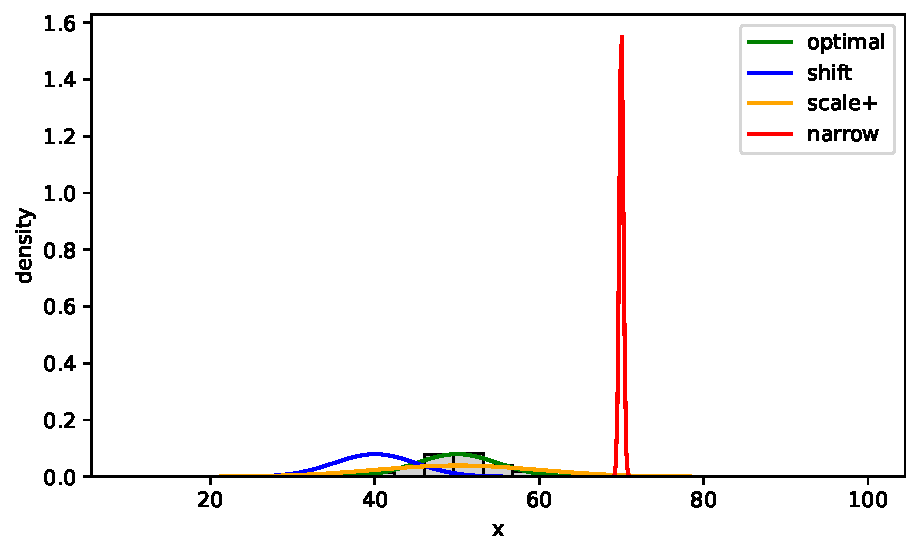
\includegraphics[width=\linewidth]{figures/ex_13_b.pdf}

		\vspace{4pt}
		{\scriptsize KLD up to additive constant:}\\
		{\scriptsize\ttfamily
		optimal: 2.11\quad shift: 4.11\\
		scale+:  2.43\quad narrow: 3398.61
		}
	\end{column}
	\end{columns}
\end{frame}

\begin{frame}[fragile]{Solution to Question (c)}
	\begin{columns}[T]
	\begin{column}{0.5\textwidth}
		\lstinputlisting{figures/ex_13_c.py}
	\end{column}
	\begin{column}{0.5\textwidth}
		\centering
		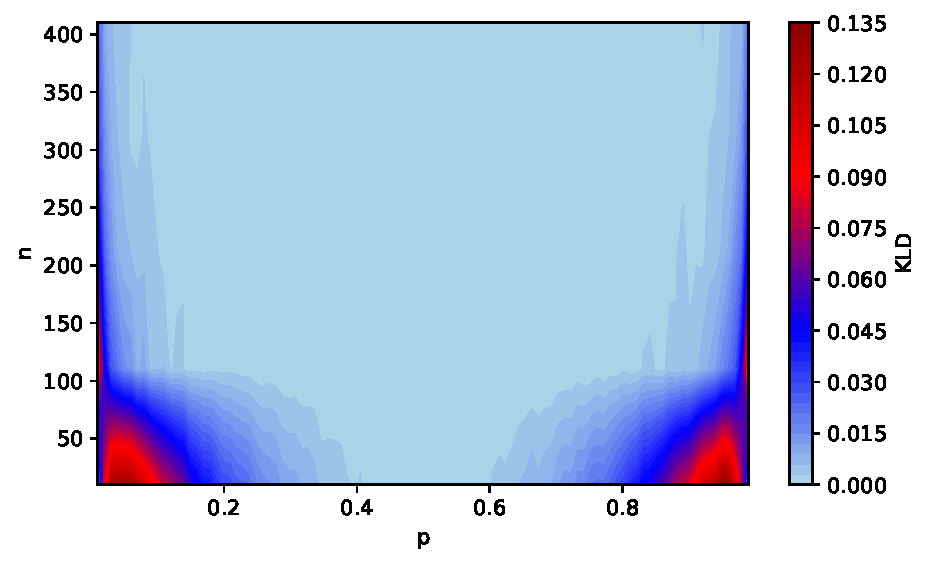
\includegraphics[width=\linewidth]{figures/ex_13_c.pdf}
	\end{column}
	\end{columns}
\end{frame}

\begin{frame}{Solution to Question (d)}
	\small
	\begin{columns}[T]
	\begin{column}{0.5\textwidth}
		\textbf{KLD over the $(n, p)$ grid:}
		\begin{itemize}
			\setlength\itemsep{6pt}
			\item Near zero for most $(n, p)$.
			\item Large near the edges $p \to 0$ or $p \to 1$ (skewed binomial).
			\item Worsens for small $n$ (CLT hasn't kicked in).
		\end{itemize}

		\vspace{6pt}
		$\Rightarrow$ Gaussian fits the binomial poorly exactly when the binomial is highly skewed or under-sampled.
	\end{column}
	\begin{column}{0.5\textwidth}
		\centering
		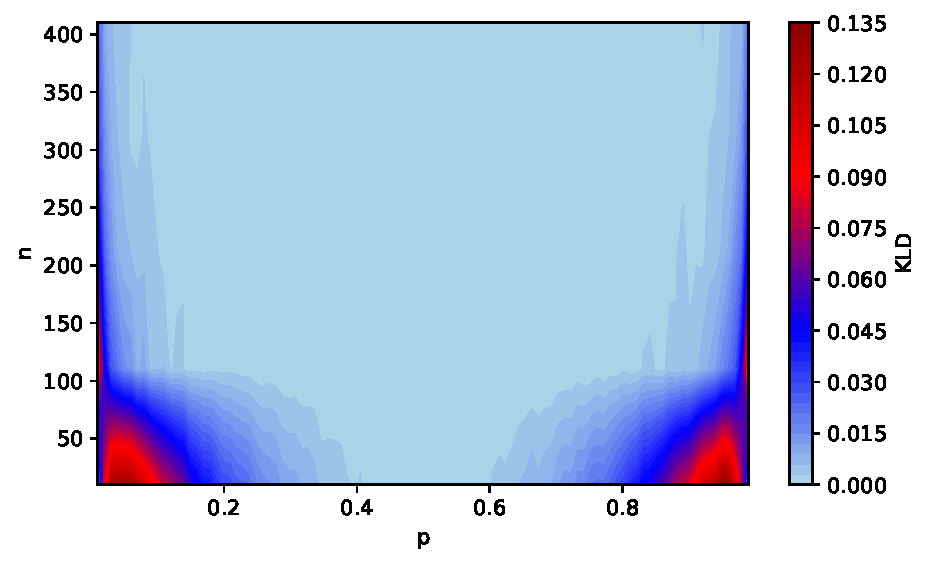
\includegraphics[width=\linewidth]{figures/ex_13_c.pdf}
	\end{column}
	\end{columns}
\end{frame}

\begin{frame}{Exercise 2: The Convexity of KL Divergence}
	Let $p$ and $q$ be the PDFs of a pair of absolutely continuous distributions. 
	
	(a) Prove that the KL divergence is convex in the pair $(p, q)$, i.e., 
	$$\kld{\lambda p_1 + (1 - \lambda) p_2 \ || \ \lambda q_1 + (1-\lambda) q_2} \leq \lambda \kld{p1 \ || \ q_1} + (1 - \lambda) \kld{p_2 \ || \ q_2},$$
	where $(p_1, q_1)$ and $(p_2, q_2)$ are two pairs of distribution and $0 \leq \lambda \leq 1$.
	
	\vspace{20pt}
	Hint: you can use the log sum inequality, namely that $(a_1 + a_2) \log \left( \frac{a_1 + a_2}{b_1 + b_2} \right) \leq a_1 \log \frac{a_1}{b_1} + a_2 \log \frac{a_2}{b_2}$ holds for $a_1, a_2, b_1, b_2 \geq 0$.
\end{frame}

\begin{frame}{Convexity: A 1D Picture}
	\begin{columns}[T]
	\begin{column}{0.55\textwidth}
		\centering
		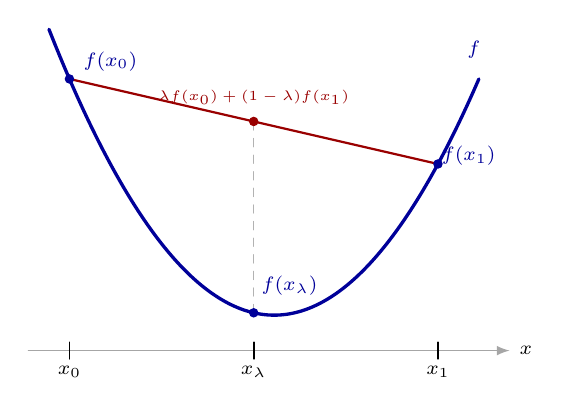
\begin{tikzpicture}[
			x=1.3cm, y=1.5cm,
			line cap=round,
			font=\scriptsize,
			>=latex,
		]
			\draw[->, semithick, gray!70] (-2.4, 0) -- (2.3, 0) node[right, black] {$x$};

			\draw[blue!60!black, very thick, smooth, samples=80, domain=-2.2:2]
				plot (\x, {(\x*\x)/2 + 0.3});

			\draw[red!60!black, thick] (-2.0, 2.3) -- (1.6, 1.58);

			\draw[gray!60, dashed, thin] (-0.2, 0.32) -- (-0.2, 1.94);

			\filldraw[blue!60!black] (-2.0, 2.3) circle (1.5pt);
			\filldraw[blue!60!black] (1.6, 1.58) circle (1.5pt);
			\filldraw[blue!60!black] (-0.2, 0.32) circle (1.5pt);
			\filldraw[red!60!black] (-0.2, 1.94) circle (1.5pt);

			\draw[semithick] (-2.0, -0.07) -- (-2.0, 0.07);
			\draw[semithick] (1.6, -0.07) -- (1.6, 0.07);
			\draw[semithick] (-0.2, -0.07) -- (-0.2, 0.07);
			\node[below=2pt] at (-2.0, 0) {$x_0$};
			\node[below=2pt] at (1.6, 0) {$x_1$};
			\node[below=2pt] at (-0.2, 0) {$x_\lambda$};

			\node[blue!60!black] at (-1.6, 2.45) {$f(x_0)$};
			\node[blue!60!black] at (1.9, 1.65) {$f(x_1)$};

			\node[blue!60!black] at (0.15, 0.55) {$f(x_\lambda)$};
			\node[red!60!black, anchor=south, font=\tiny] at (-0.2, 2.0) {$\lambda f(x_0) + (1-\lambda) f(x_1)$};

			\node[blue!60!black] at (1.95, 2.55) {$f$};
		\end{tikzpicture}
	\end{column}
	\begin{column}{0.45\textwidth}
		\footnotesize
		For $\lambda \in [0, 1]$, let $x_\lambda = \lambda x_0 + (1-\lambda) x_1$. Convexity of $f$ means:
		\[
			f(x_\lambda) \,\leq\, \lambda f(x_0) + (1-\lambda) f(x_1).
		\]
		\begin{itemize}
			\setlength\itemsep{2pt}
			\item $x_\lambda$ is a convex combination of $x_0$ and $x_1$.
			\item $\lambda f(x_0) + (1-\lambda) f(x_1)$ is the chord value at $x_\lambda$.
			\item The chord lies above the curve.
		\end{itemize}

		\vspace{4pt}
		In Exercise 2:
		\begin{itemize}
			\setlength\itemsep{2pt}
			\item Each ``$x$'' is a pair $(p, q)$ of distributions.
			\item $f$ is the KL divergence $D_{KL}(p \,\|\, q)$.
		\end{itemize}
	\end{column}
	\end{columns}
\end{frame}

\begin{frame}{Solution to Question (a)}
	\small
	\begin{align*}
		& \kld{\lambda p_1 + (1 - \lambda) p_2 \ || \ \lambda q_1 + (1-\lambda) q_2} \\
		\only<2->{&= \int_\Xspace \left( (\lambda p_1(x) + (1 - \lambda) p_2(x)) \log \frac{\lambda p_1(x) + (1 - \lambda) p_2(x)}{\lambda q_1(x) + (1 - \lambda) q_2(x)} \right) \mathrm{d}x \\}
		\only<3->{&\leq \int_\Xspace \left( \lambda p_1(x) \log \frac{p_1(x)}{q_1(x)} + (1-\lambda) p_2(x) \log \frac{(1 - \lambda) p_2(x)}{(1-\lambda) q_2(x)} \right) \mathrm{d}x \quad (\text{Use hint}) \\}
		\only<4->{&= \lambda \int_\Xspace \left(p_1(x) \log \frac{p_1(x)}{q_1(x)} \right) \mathrm{d}x + (1 - \lambda) \int_\Xspace \left( p_2(x) \log \frac{p_2(x)}{q_2(x)}\right) \mathrm{d}x \\}
		\only<5->{&= \lambda \kld{p_1 \ || \ q_1} + (1 - \lambda) \kld{p_2 \ || \ q_2}.}
	\end{align*}
\end{frame}


\end{document}
